\chapter{METHODS}
\section{Model Searching Method}
  %Untuk mencari solusi optimisasi pendeteksian objek kecil YOLOv7 yang terbaik, akan dilakukan penambahan atau perubahan \emph{bag-of-freebies}, \emph{bag-of-specials}, dan arsitektur YOLOv7.
  %Setiap modifikasi-modifikasi itu akan diaplikasikan secara independen dan kombinatif.
  %Yang dimaksud dengan kombinatif adalah modifikasi-modifikasi akan dikombinasikan menjadi 1 model YOLOv7.

  %Setiap kombinasi modifikasi, independen atau tidak, akan diuji kemampuannya mendeteksi objek \emph{airborne}.
  %Solusi optimisasi terbaik akan ditentukan berdasarkan metrik $AP_{50}$.
  %Subbab \ref{section:modificationcandidates} akan membahas tentang kandidat modifikasi-modifikasi yang dapat dilakukan.

  %Tahapan pencarian solusi optimisasi sendiri dapat dibagi menjadi enam tahap.
  %Tahap-tahap tersebut adalah Persiapan Dataset, Pembuatan \emph{Auto-trainer}, Pembuatan Konfigurasi Modifikasi, \emph{Training Model}, Analisis, dan Pemilihan Model Terbaik.
  %Urutan pengerjaan dari tahap-tahap ini dapat dilihat pada Gambar \ref{fig:metodologi}.
To find the best model for detecting small objects, trial and error will be performed by
adding or changing architecture, bag-of-specials, or bag-of-freebies of YOLOv7.
These modifications will be tried out independently and combinatively.

Every modification will be tested on its ability to detect airborne object.
The best model will be selected based on $mAP@50$ metric.
This metric was chosen instead of $mAP@[50:95]$ because we don't expect for the model to be able to predict a tightly fit
bounding boxes for small object and consider a loose 50\% coverage IoU is good enough.

The model searching method is comprised of six steps.
These steps are dataset preparation, develop training system, create modification model configuration,
training the model, analysis, and model selection. 
Figure \ref{fig:methods} shows the order these steps will be executed.

\begin{figure}[H]
  \centering
  \small
  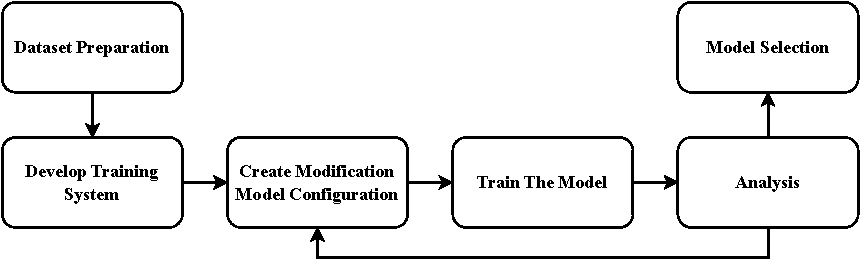
\includegraphics[width=.9\textwidth]{figures/methods.pdf}
  \caption{Search Steps}
  \label{fig:methods}
\end{figure}
\vspace{-1ex}
  %insert diagram modifikasi here
  %Menyiapkan dataset, Membuat \emph{auto-trainer}, Membuat konfigurasi-konfigurasi modifikasi, Melatih model-model YOLOv7 yang sudah dimodifikasi,
  %Menganalisis performa hasil modifikasi YOLOv7, dan Pemilihan model modifikasi YOLOv7 dengan skor mAP terbaik.

  %Pada tahap persiapan dataset, akan dilakukan pengunduhan dataset dari \textcite{aot_dataset}.
  %Gambar-gambar pada dataset ini kemudian akan di-\emph{sampling} dan didistribusikan menjadi dataset \emph{training}, validasi, dan pengujian.
  %Pada pendistribusian dataset ini juga akan dilakukan \emph{balancing} antar kelas dan dataset positif negatif.
  %\emph{Balancing} dilakukan agar tidak ada kelas yang mendominasi pada dataset.

  %Selanjutnya, di tahap pembuatan \emph{auto-trainer}, akan dilakukan pembuatan program yang dapat dengan otomatis membangun dan melatih \emph{neural network} modifikasi YOLOv7.
  %Pembuatan \emph{auto-trainer} ini dilakukan agar proses-proses pengerjaan tahapan-tahapan selanjutnya menjadi dapat dilakukan dengan lebih mudah.

  %Setelah itu, akan dilakukan pembuatan konfigurasi-konfigurasi modifikasi.
  %Konfigurasi modifikasi YOLOv7 akan dibuat agar dapat diinputkan pada \emph{auto-trainer}.
  %Konfigurasi modifikasi akan berisi kombinasi modifikasi-modifikasi yang ada pada subbab \ref{section:modificationcandidates}.

  %Tahapan selanjutnya adalah \emph{Training} model.
  %Pada tahap ini, konfigurasi-konfigurasi modifikasi pada tahapan sebelumnya akan dibangun dan kemudian dilatih.
  %Model akan dilatih \emph{from scratch}. Dengan kata lain, model tidak akan dilatih dengan menggunakan \emph{pre-trained weights}.
  %Hasil dari tahap ini adalah \emph{weights neural network} modifikasi YOLOv7, histori pelatihannya, dan metrik-metriknya pada dataset uji.

  %Pada tahap analisis, hasil dari tahap sebelumnya akan dianalisis untuk mencari tahu performa model-model hasil modifikasi.
  %Analisis juga dilakukan untuk menemukan \emph{gap} kandidat modifikasi lain yang masih bisa dieksplorasi untuk meningkatkan kemampuan pendeteksian objek kecil YOLOv7.
  %Ketika suatu kandidat modifikasi seperti itu ditemukan, maka akan dilakukan kembali pembuatan konfigurasi modifikasi untuk menguji kandidat modifikasi baru tersebut.

To conduct this research, we first have to prepare the dataset.
First, the dataset will be downloaded from \textcite{aot_dataset}.
Then, the labels of the dataset will be converted to darknet or COCO format.
Next, the dataset will be sampled into training set, validation set, and test set.
The sampling will be done in a way that balances the number classes in each set so
that there will be no dominating class during training.
  
The next thing to do is to develop a training system.
The purpose of this system is to make the training process easily conducted and monitored.
This system will include features such as train fail notification, train queueing, and alert the user
when the computer overheats.

Moving on, we have model configuration creation. Here we will create a model configuration file based on the 
modification that we want to try. The modification configurations will be made according to the modification
candidates listed in section \ref{section:modificationcandidates}.

The next step is to train the model.
The model configurations that was made in previous step will be built and trained from scratch (no pre-trained weights).
In this step, the weights of the neural network, training history, and performance metrics will be generated for analysis.

In the analysis step, we will analyze the performance of the modified YOLOv7.
This step is done to find other candidate of modification that might work.
If such modification candidate was found, we will go back to create the model configuration, 
and then train the modification.

Finally, in the last step we will select the best model.
We will select the model with the best performance among the modified YOLOv7 models.
The model selection will be done based on $mAP@50$ metric, with constraint in inference latency.
The model that qualify for selection must be able to perform inference with speed of atleast 10 FPS in a consumer GPU Nvidia RTX 2080Ti.
  %Tahapan terakhir adalah pemilihan model terbaik.
  %Pada tahapan ini akan dipilih model yang memiliki performa terbaik dari antara model-model hasil modifikasi lainnya.
  %Pemilihan model akan dilakukan dengan berdasarkan pada skor mAP tertinggi.
  %Untuk mempertahankan solusi optimisasi yang dapat melakukan deteksi secara \emph{real time}, model yang akan dipilih adalah model yang dapat melakukan deteksi yang cukup cepat pada \emph{edge} GPU.


\section{Modification Candidates}
\label{section:modificationcandidates}
  \subsection{Mosaic Augmentation}
  As discussed in section \ref{section:mosaic_study}, mosaic augmentation was able to increase the detection accuracy of small objects
  on many object detection neural networks. For this reason, we will experiment by training YOLOv7 with and without  mosaic augmentation.
    %Seperti yang dibahas pada subbab \ref{section:mosaic_study}, augmentasi mosaic pada dataset mampu meningkatkan akurasi deteksi objek-objek kecil dari model.
    %Oleh karena itu, akan dilakukan eksperimen menambahkan augmentasi mosaik pada YOLOv7 untuk melihat apakah augmentasi ini akan meningkatkan akurasi, khususnya pada dataset objek kecil.
  \subsection{Pre-training Anchor Recalculation}
    %Yang dimaksud dengan rekalkulasi \emph{anchor on-training}  adalah ketika ukuran-ukuran \emph{anchor box} direkalkulasi pada saat training.
    %Berbeda dengan \emph{clustering pre-training} seperti pada YOLOv2 \parencite{yolov2}, ukuran-ukuran \emph{anchor} akan di-\emph{learning} bersama dengan pendeteksi objeknya.
    %Untuk melakukan hal ini, digunakan algoritma optimisasi \emph{anchor box} yang mirip dengan algoritma \textcite{anchoropt}.
    %Pada bagian \emph{head}, akan ditempelkan suatu layer yang akan mengoutputkan faktor \emph{rescaling} dari tiap \emph{anchor box}.
    %Bagian tersebut akan di-\emph{training} bersama dengan YOLOv7 \emph{anchor box} akan teroptimisasi tidak hanya pada dataset, namun pada keseluruhan \emph{neural network} juga.

    %Anchor yang disediakan pada kode implementasi dari YOLOv7 merupakan anchor yang dikalkulasi untuk mengoptimisasi deteksi pada dataset
    %COCO2017. Dengan pertimbangan bahwa distribusi dataset yang akan digunakan pada penelitian ini berbeda dari objek general di COCO2017,
    %maka anchor harus direkalkulasi. Dengan melakukan rekalkulasi anchor, tiap layer head pada YOLOv7 akan dengan lebih mudah mem-\emph{fit}
    %objek-objek yang ada pada gambar.
  In the implementation code of YOLOv7, the anchors provided was calculated based on COCO2017 dataset.
  We assume that the dataset distribution of airborne objects to be greatly different from COCO2017.
  As such, the anchors must be recalculated for faster learning. This recalculation will be conducted
  using k-means algorithm. One problem however is that k-means might fail to cluster the dataset into 
  the amount of anchors that we needed. To tackle this, we might have to cluster it in logarithmic coordinates. 

  \subsection{Replacing Localization Loss to Extended IoU}
  \begin{figure}[H]
      \centering
      \begin{subfigure}[][][t]{0.3\textwidth}
        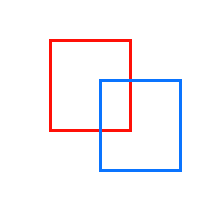
\includegraphics[width=1\linewidth]{figures/iounot0.png}
        \caption{$IoU > 0$ when 2 boxes intersect}
        \label{fig:iouexist}
      \end{subfigure}\hfill
      \begin{subfigure}[][][t]{0.3\textwidth}
        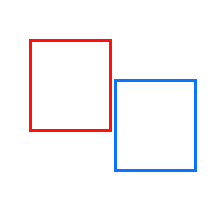
\includegraphics[width=1\linewidth]{figures/iou0near.png}
        \caption{$IoU = 0$ when 2 boxes does not intersect}
        \label{fig:iou0near}
      \end{subfigure}\hfill
      \begin{subfigure}[][][t]{0.3\textwidth}
        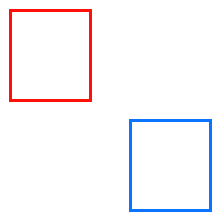
\includegraphics[width=1\linewidth]{figures/iou0far.png}
        \caption{$IoU = 0$ when 2 boxes does not intersect and far away}
        \label{fig:iou0far}
      \end{subfigure}
      \caption{Cause of IoU vanishing gradient}
      \label{fig:iouvanishinggrad}
  \end{figure}
  Extended-IoU (EIoU) is a modification of IoU that are used in neural networks to tackle
  the problem of vanishing gradient \parencite{eiou}. 
  IoU are known to cause vanishing gradient problem due to its behavior when two bounding boxes are not intersecting.
  When 2 boxes $A$ and $B$ are not intersecting, the area of intersection ($A\cap B$) would always be 0.
  This value doesn't give any information whether the boxes are far apart (Figure \ref{fig:iou0far}) or 
  near but not intersecting (Figure \ref{fig:iou0near}).
  To solve this, loss involving $IoU$ are usually paired with some regularization terms.
  For example \textcites{giou}{diou_ciou} proposed $GIoU$, $DIoU$, and $CIoU$.
  
  YOLOv7 itself is using $CIoU$ for its localization loss. $CIoU$ is just regular $IoU$
  that is paired with distance and box aspect ratio regularization terms.
  The problem of these kinds of regularized IoU is that when the boxes intersect, it does not
  behave like IoU anymore. $GIoU$, $DIoU$ and $CIoU$ have residue of their regularization when
  the boxes intersect. Metrics used to evaluate object detection
  algorithms depend on IoU (\textit{e.g.\ mAP}).
  For this reason \textcite{eiou} designed EIoU. The main appeal of EIoU
  is that it behave exactly like IoU when the boxes intersect and gives non-positive value when the
  boxes do not intersect.
  By behaving exactly like IoU, it is hoped that the model would perform better on the metrics.


    %\emph{Extended} IoU (EIoU) merupakan salahsatu modifikasi dari
    %IoU yang dibuat untuk menyelesaikan permasalahan \emph{vanishing gradient}
    %pada IoU \parencite{eiou}. Hal yang menyebabkan IoU bermasalah dengan \emph{vanishing gradient}
    %adalah nilai dari IoU yang selalu menjadi 0 ketika 2 \emph{bounding box} tidak beririsan.
    %Permasalahan ini diselesaikan oleh EIoU dengan memberikan nilai negatif untuk 
    %bounding box yang tidak beririsan, sehingga neural network dapat mengoptimasi loss function $-EIoU$.
    %Teknik konveksikasi juga dapat dilakukan dengan mengoptimasi $(1-EIoU)^2$

    %YOLOv7 sendiri menggunakan CIoU sebagai localization loss. CIoU juga merupakan suatu solusi
    %dari permasalahan \emph{vanishing gradient}. CIoU menambahkan suku jarak antar bounding box 
    %dan kecocokan \emph{aspect ratio} antar boundingbox pada IoU. Keunggulan EIoU daripada CIoU
    %adalah EIoU akan bertingkah seperti IoU ketika bounding box beririsan. Karena metrik-metrik
    %yang digunakan untuk mengukur kemampuan deteksi dilakukan berdasarkan IoU, dianggap akan
    %lebih baik jika loss yang digunakan sama seperti metriknya \parencite{eiou}.

  \subsection{Utilizing Earlier Feature Map Stage}
    %\begin{figure}[ht]
    %  \centering
    %  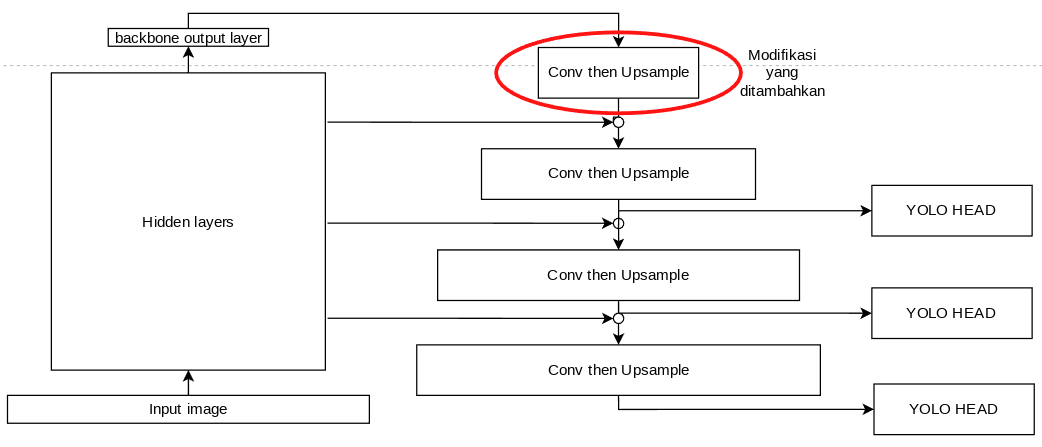
\includegraphics[scale=0.5]{figures/add-more-upsampling.png}
    %  \caption{Menambah \emph{upsampling} pada \emph{neck}}
    %  \label{fig:neckaddupsampling}
    %\end{figure}

  \begin{figure}[H]
    \centering
    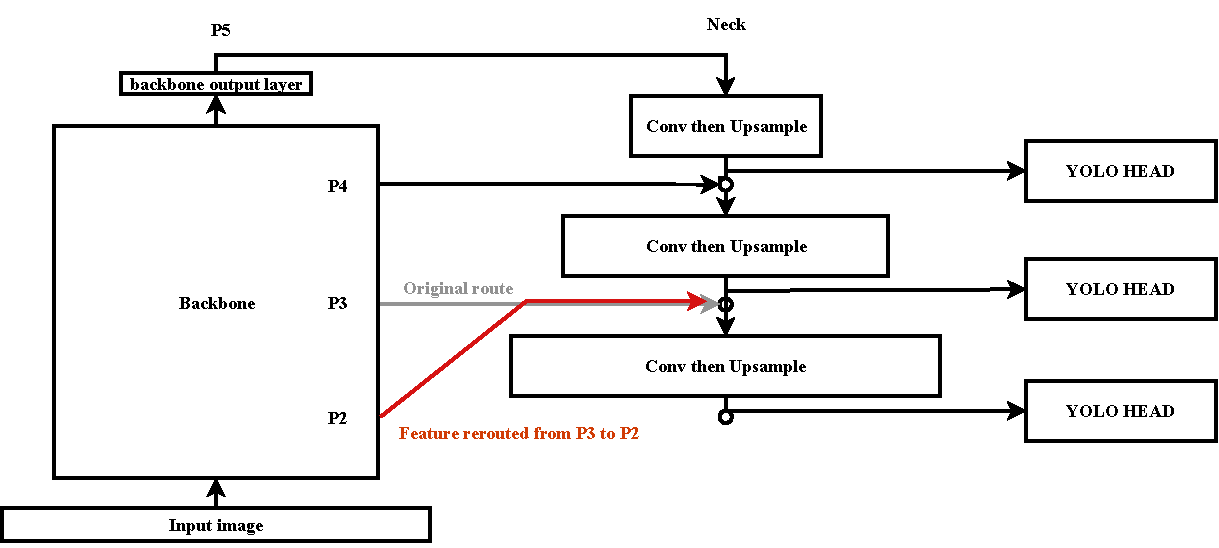
\includegraphics[width=.9\textwidth]{figures/neck-move-back.pdf}
    \caption{Rerouting Neck Connection to Earlier Stage}
    \label{fig:neckmoveback}
  \end{figure}
  In a deep neural network, the extracted feature/abstraction of the data become more prominent
  as the input data passes through deeper layers. However, information loss also increases in the
  deeper layer. For small object detection, information is crucial. There is a posibility the features
  of small objects are lost as the data propagates through the network.
  
  If we view it in a data path network design perspective, the greater the length of the path from input
  to output, the more information will be lost. Therefore, we propose to reroute the orignal connection from
  backbone to the neck to an earlier stage of inference. For example, YOLOv7 take feature maps from P3, P4, and P5
  scales of the backbone, we can reroute the connection from P3 to P2 as shown in Figure \ref{fig:neckmoveback}.
  %Seperti pada penelitian-penelitian terkait di subbab \ref{section:relatedwork}, modifikasi \emph{neck} dapat dilakukan untuk meningkatkan akurasi pendeteksian objek kecil.
  %Modifikasi koneksi \emph{neck} ke \emph{backbone} dapat dilakukan dengan memindahkan sumber feature map untuk beberapa layer neck lebih jauh ke belakang seperti pada Gambar \ref{fig:neckmoveback}.
  %%Penambahan layer upsampling dapat membuat neural network untuk mendapatkan feature-map yang lebih detail sehingga dapat melakukan pendeteksian objek kecil dengan lebih baik.
  %Pemindahan sumber feature map ke belakang dapat dilakukan untuk mengantisipasi fitur objek kecil yang bisa saja hilang ketika layer neural network semakin dalam.
  %Dengan memindahkannya lebih ke belakang, YOLOv7 akan melakukan deteksi dengan memanfaatkan fitur yang abstraksi yang lebih rendah tetapi sedikit informasi yang hilang.
  \subsection{Additional YOLO Head}
  \begin{figure}[H]
    \centering
    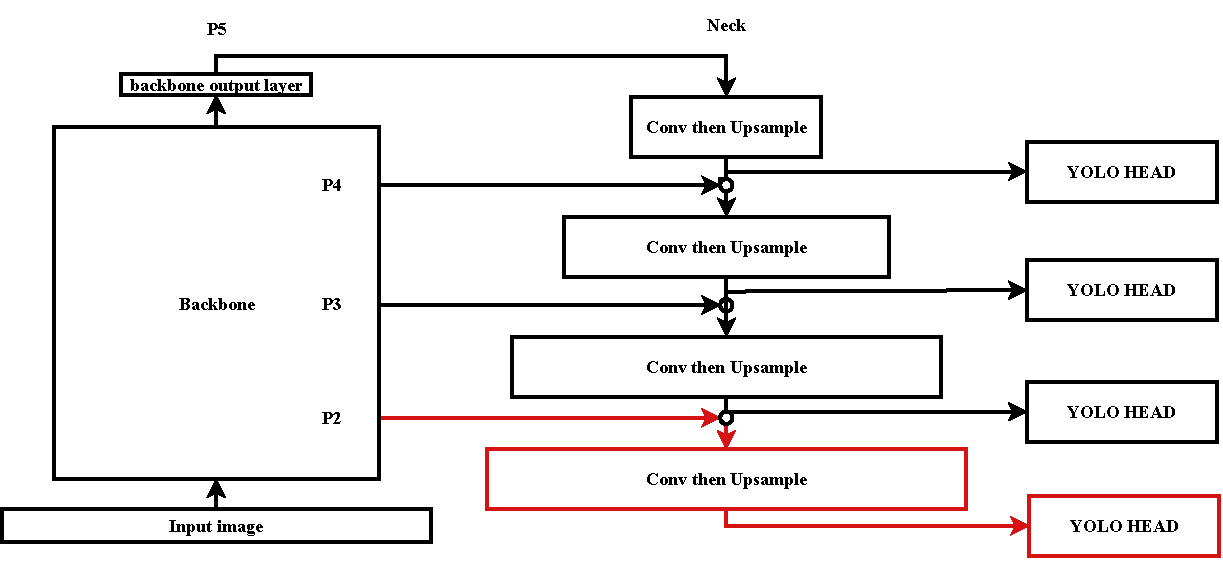
\includegraphics[width=.9\textwidth]{figures/addmorehead.pdf}
    \caption{Adding an Extra Head Layer}
    \label{fig:addmorehead}
  \end{figure}
  An additional YOLO head means an extra stage of detection.
  With more stage of detection, the large variance of the objects in the dataset can be learned.
  This is especially good for \textcite{aot_dataset} where the area of the bounding boxes in the dataset
  can be orders of magnitude apart (see section \ref{section:dataset}).
  
  %%Penambahan YOLO head dapat membuat YOLOv7 melakukan deteksi pada skala yang lebih banyak.
  %%Hal ini akan berpengaruh pada kemampuan pendeteksian objek kecil.
  %%Dengan melakukan pendeteksian pada skala yang lebih banyak, YOLOv7 dapat mendeteksi objek yang besar maupun kecil.
  %Perhatikan bahwa penambahan YOLO Head akan diikuti dengan penambahan \emph{layer upsampling} pada \emph{neck} seperti di Gambar \ref{fig:addmorehead}.

  \subsection{Replace YOLO Head to YOLOX's Decoupled Anchor-free Head}
  \begin{figure}[H]
    \centering
    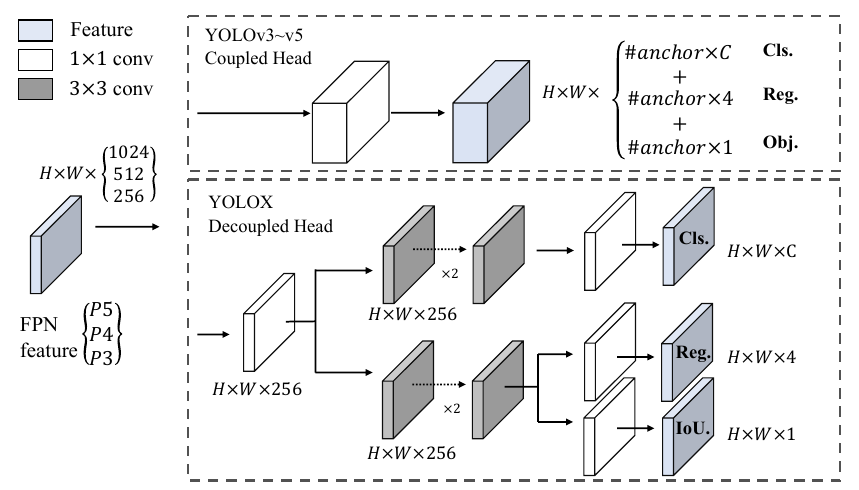
\includegraphics[width=0.8\textwidth]{figures/anchorfree-yolox.png}
    \caption{Decoupled Anchor-free Head in YOLOX compared to Coupled Head in mainstream YOLO}
    \label{fig:anchorfree}
  \end{figure}

  YOLOv6 and YOLOX used a different kind of head layer compared to usual YOLO \parencites{yolox}{yolov6}. 
  In mainstream YOLO, prediction for bounding box and classes are both calculated on the same layer.
  With decoupled anchor-free head, the layers are separated for class prediction and bounding box prediction, and
  bounding box prediction are done using 4 value without anchor as seen on Figure \ref{fig:anchorfree}. 
  Using decoupled anchor-free head gives us 2 advantages. 1) Reducing the amount of design parameters as 
  we don't have to introduce anchor boxes to the model. 2) Reducing the complexity of interpreting prediction
  result. Advantage (1) is especially enticing. There is a possibility of us introducing bad priors to the neural
  network by poorly clustering anchor boxes. By having a model that less dependent on prior, we can reduce such possibility.

  A thing to consider when applying decoupled anchor-free head to YOLOv7 is the label assigner. YOLOv7 and YOLOX uses SimOTA as its default
  label assigner. However, \textcite{yolov6} YOLOv6 uses Task-aligned Assigner (TAL) for its label assigner. They reported that TAL performs
  better than SimOTA. Therefore, in applying decoupled anchor-free head, it might be better to use TAL as label assigner.
  %Decoupled head gives us 2 advantages. 
  %1) Reducing the amount of

  \subsection{Partitioning Image}
  \begin{figure}[H]
    \centering
    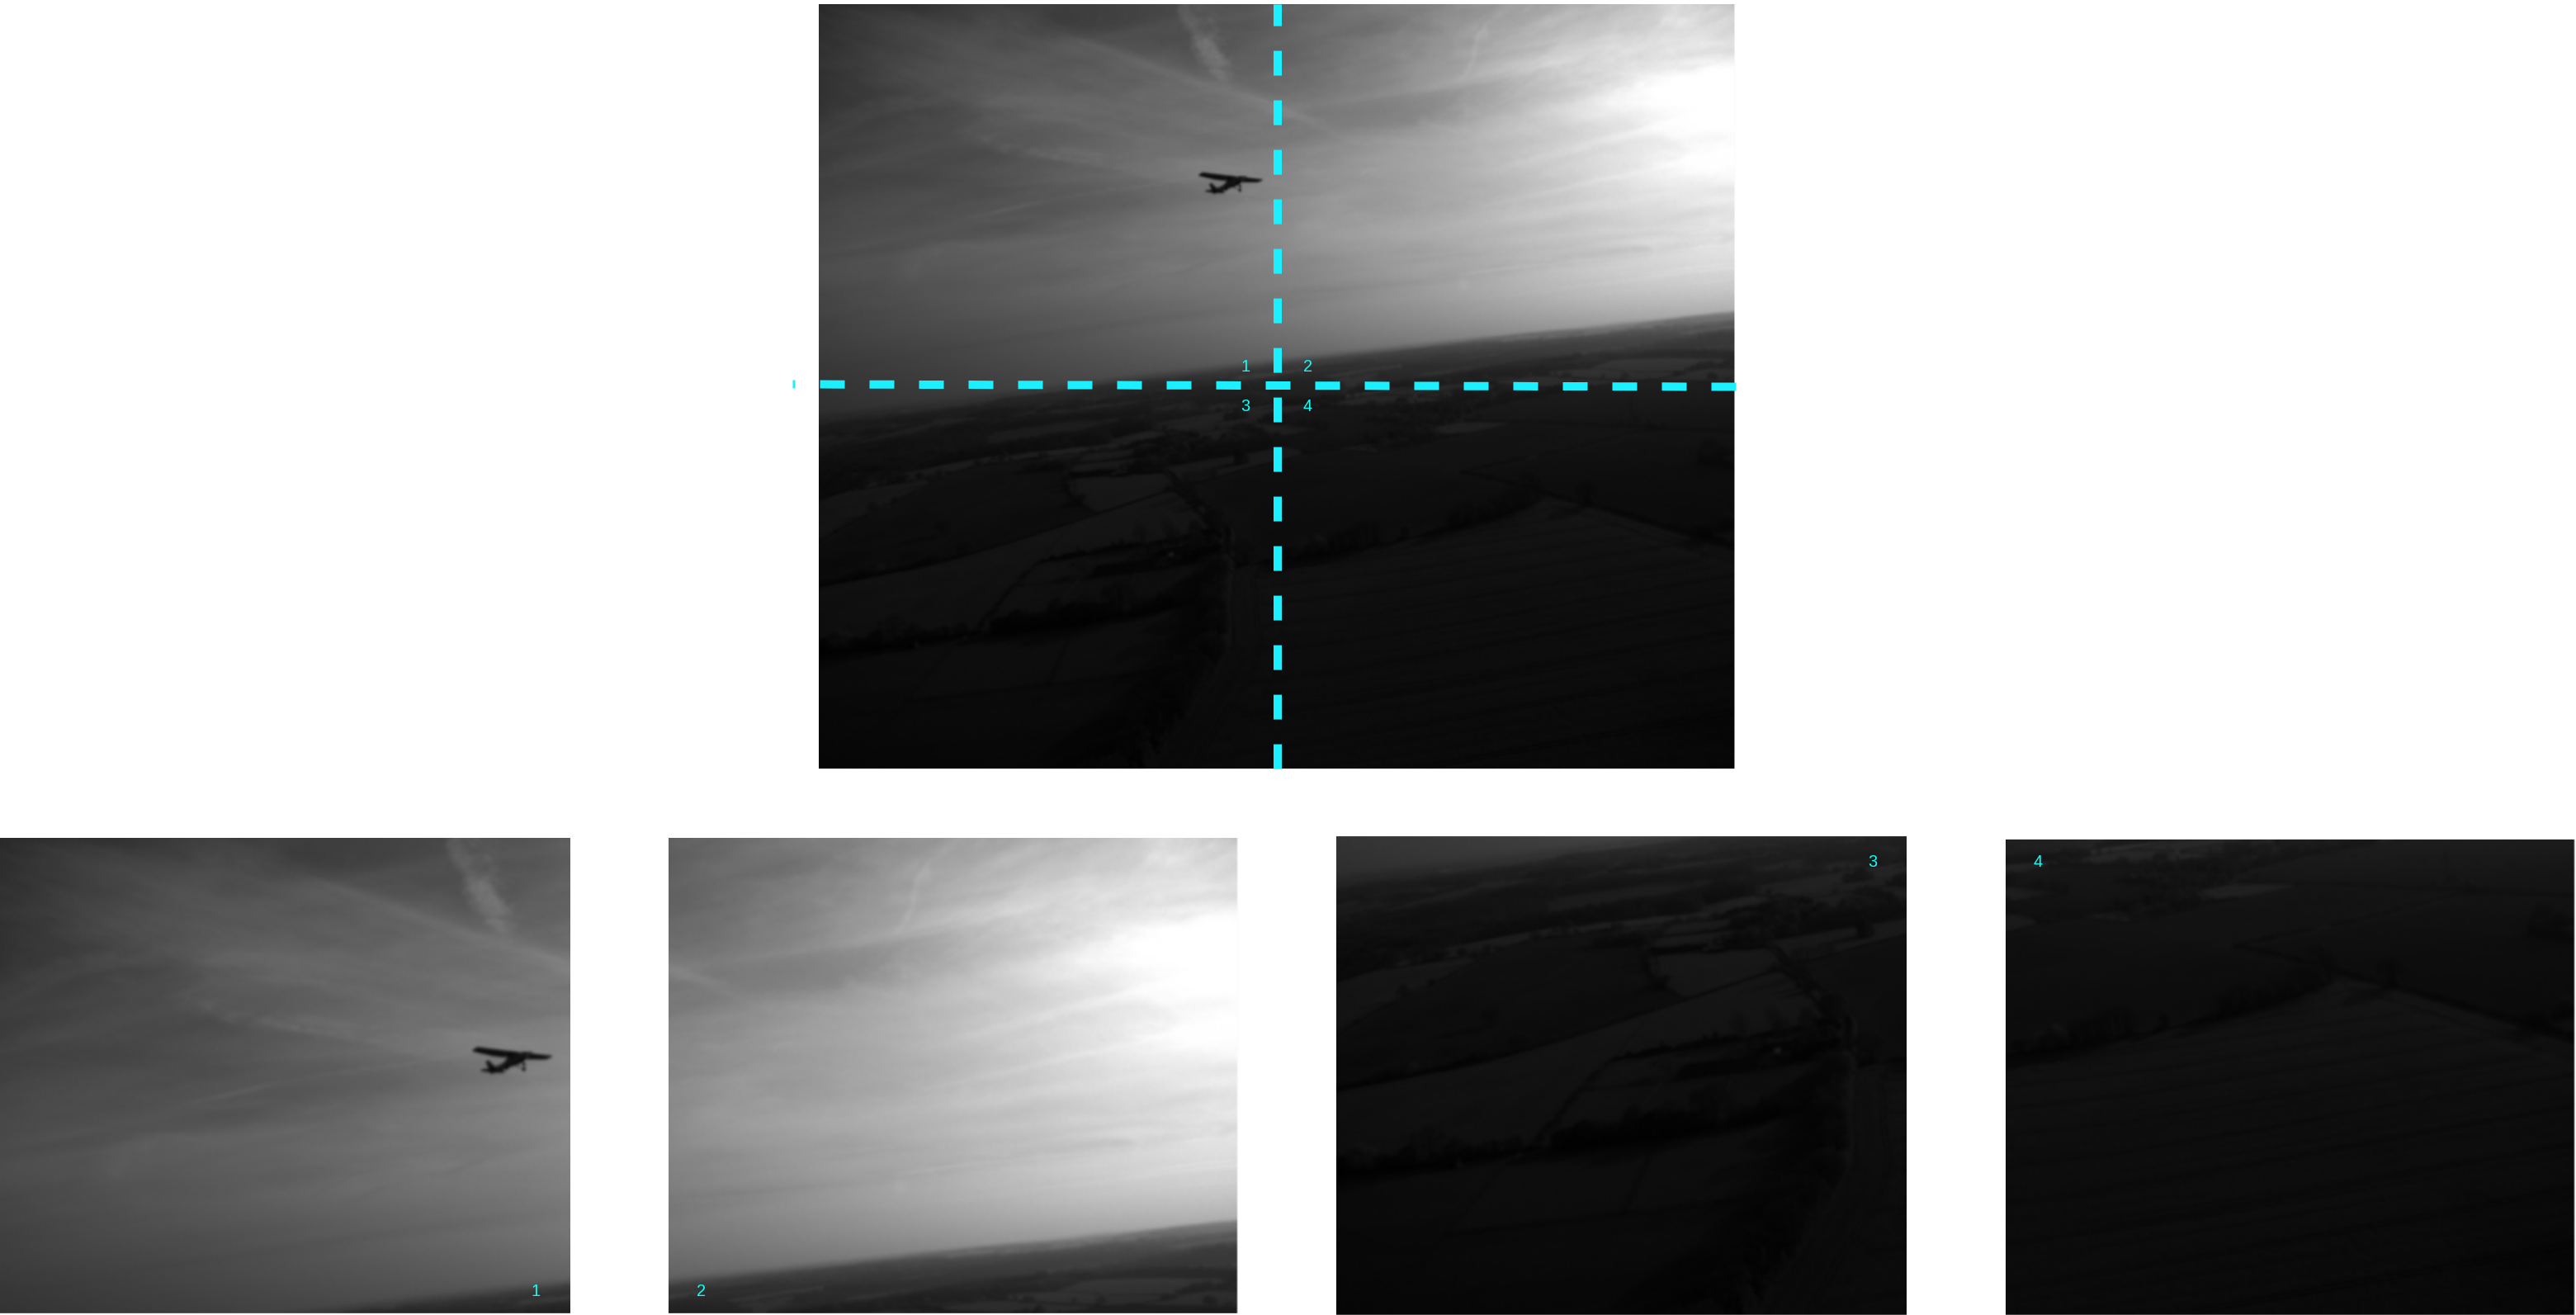
\includegraphics[width=0.9\textwidth]{figures/imagepartition.png}
    \caption{An Image Partitioned to 4 Images}
    \label{fig:imagepartition}
  \end{figure}
  Partitioning the image can significantly improve the accuracy of small object detection.
  The partitioning process involves cropping the original image into smaller sections, thereby avoiding excessive downscaling of the image before feeding it into the neural network.
  This approach allows the network to retain finer details and preserve the integrity of small objects, ultimately leading to more accurate detection results.
  By breaking down the image into manageable segments, the network can focus on individual regions of interest and capture the features of small objects with greater precision. 

  One challenge associated with partitioning images is the potential increase in inference latency.
  When an image is partitioned into multiple sections, the neural network needs to perform separate detections on each partition.
  As a result, the inference time is multiplied by the number of partitions.
  For instance, if we divide an image into four parts, the network will have to carry out four separate detections, leading to a significant increase in latency. 
  %Pada YOLOX, \emph{coupled anchor head} seperti pada arsitektur YOLO pada umumnya diganti dengan \emph{decoupled anchor-free head} \parencite{yolox}.
  %Keuntungan dari model anchor-free adalah kita tidak perlu mendefinisikan \emph{anchor} sebelum melakukan training sehingga mengurangi beberapa proses
  %tuning heuristik seperti rekalkulasi anchor. Memakai \emph{head} yang anchor free juga memberi kompleksitas proses training dan pendekodean output model.
  %\cite{yolox} melaporkan peningkatan pada akurasi dan pengurangan parameter sehingga mempercepat lama deteksi.
  %Oleh karena hal-hal tersebut, mencoba memakai \emph{head anchor-free} di YOLOv7 baik untuk dicoba.
    
\section{Instruments}
\label{section:instrument}
To conduct this research, we will be using a computer with the following specification:
\begin{itemize}[noitemsep,topsep=0pt,leftmargin=.1\textwidth,rightmargin=.1\textwidth]
  \item CPU \hfill Intel® Core™ i5-9400F CPU @ 2.90GHz
  \item GPU \hfill Nvidia Geforce RTX 2080 Ti
  \begin{itemize}[noitemsep,topsep=0pt]
    \item[] Memory \hfill 11 GB
    \item[] CUDA Compute Capability \hfill 7.5
  \end{itemize}
  \item RAM \hfill 12 GB
  \item Hard Drive Available Memory \hfill 1.3 TB
  \item Operating System \hfill Ubuntu 20.04
  \item Cuda Toolkit Version \hfill 11.7
  \item PyTorch Version \hfill 1.13.1
\end{itemize}

\section{Pilot Test}
To ensure the reliability of the instruments, and to find the instrument-induced constraint, we performed A
pilot test.
In this pilot test, we trained several YOLOv7 models with varying input sizes with a dummy dataset for 300 epochs.
The dummy dataset have the same dimension as the \textcite{aot_dataset}.
The results are presented in Table \ref{tbl:pilot}. 
\begin{table}[H]
  \centering
  \captionof{table}{Pilot Test Training}
  \label{tbl:pilot}
  \vspace{-1ex}
  \begin{adjustbox}{width=\textwidth}
    \begin{tabular}{ l l c c c c}
  \toprule[1.5pt]
  No & Model                                       &  Input Size   &Training Time (300 epochs)    &VRAM Usage & Average GPU Temperature \\
  \midrule
  0  & \texttt{YOLOv7}                             &     640       & 4.0h                         &4.5GB          &  82                     \\
  1  & \texttt{YOLOv7 batch-size=2}                &     640       & 2.5h                         &6.5GB          &  82                     \\
  2  & \texttt{YOLOv7}                             &     960       & 4.7h                         &6.5GB          &  84                     \\
  3  & \texttt{YOLOv7}                             &     1600      & 20h                          &9.5GB          &   84                    \\
  4  & \texttt{YOLOv7}                             &     2000      & N/A                          &Out of Memory  &                         \\
  5  & \texttt{YOLOv7-d6}                          &     1600      &                              &10GB           &  85                     \\
  6  & \texttt{YOLOv7-w6}                          &     1600      & N/A                          &10.5GB         &                         \\
  7  & \texttt{YOLOv7-e6}                          &     1600      & N/A                          &Out of Memory  &                         \\
  8  & \texttt{YOLOv7-e6e}                         &     1600      & N/A                          &Out of Memory  &                         \\
  %\midrule
  %   & Improvement                                 &              & \textbf{\textcolor{red}{-6\%}} &TBA\\
  \bottomrule[1.5pt]
\end{tabular}
  \end{adjustbox}
\end{table}

From Table \ref{tbl:pilot}, we want to pick a baseline model to apply our modification.
Since we want to persist the features of the $2048\times 2448$ px images, we pick the 
largest input size the machine can handle but still able to give enough room for some 
changes in architecture. For this reason, we picked YOLOv7 with input size 1600 and batch size 1
as the baseline.

\section{Dataset Preparation}
\label{section:dataset}

  \subsection{Dataset Source}
  \label{section:datasetsource}
  Dataset containing annotated images of airborne objects can be obtained from \textcite{aot_dataset}.
  This dataset is hosted in an AWS S3 Bucket.
  The dataset consist of several Unmanned Aerial Vehicle (UAV) flights' frame-by-frame camera capture.
  There are 7 classes in the dataset but most there are 3 dominating classes.
  The size of the dataset and its class distribution can be seen on Figure \ref{tbl:datasettraintest} and
  \ref{tbl:datasetclasses} respectively.
  %Dataset untuk objek-objek \emph{airborne} didapatkan dari \textcite{aot_dataset} dan dihost pada suatu server AWS S3 Bucket.
  %Dataset ini berisi video-video monokromatik penerbangan UAV.
  %Terdapat 4 kelas pada dataset ini yaitu pesawat, helikopter, burung, dan \emph{other}.
  %Distribusi dataset training dan uji dapat dilihat pada tabel \ref{tbl:datasettraintest} sedangkan distribusi kelas dari dataset dapat dilihat pada Tabel \ref{tbl:datasetclasses}.
  \begin{table}[H]
    \centering
    \captionof{table}{Original Dataset Splits}
    \label{tbl:datasettraintest}
    
\begin{table}[H]
  \centering
  \captionof{table}{Distribusi Dataset Training dan Test}
  \label{tbl:datasettraintest}
  \begin{tabular}{|c|c|c|c|c|}
    \hline
    Pembagian & Ukuran (TB) & Sekuen penerbangan & Jumlah Gambar & Jumlah Label\\
    Dataset &  & UAV &  & \\
    \hline
    Training & 11,3 & 4154 & 4975765 & 2891891\\
    \hline
    Validation + Test &2.1 &789 & 943852 & 496075\\
    \hline
    Total &13,4 &4943 & 5919617 & 3387966\\
    \hline
  \end{tabular}
\end{table}
  \end{table}
  \begin{table}[H]
    \centering
    \captionof{table}{Dataset' Objects Classes Distribution}
    \label{tbl:datasetclasses}
    \begin{tabular}{ c c c c c c }
  \toprule[1.5pt]
  Splits & Total Objects & Airplane & Helicopter & Bird & \emph{Other 4 Classes}\\
  \midrule
  Training & 2,89 M & 0,79 M& 1,22 M& 0,33 M& 0,54 M\\
  Validation + Test &0,50 M &0,13 M & 0,17 M&0,06 M&0,14 M\\
  \midrule
  Total &3,39 M &0,92 M & 1,39 M&0,39 M&0,69 M\\
  \bottomrule[1.5pt]
\end{tabular}
  \end{table}
  %Kebanyakan \emph{bounding box} pada dataset berukuran sangat kecil.
  %Distribusi dari luas \emph{boudning box} dapat dilihat pada gambar \ref{fig:areadist}.
  %Perhatikan pada gambar tersebut, sumbu x menggunakan skala logaritmik.
  %Sebagai referensi, luas dari tiap frame itu sekitar $5\times10^16 px^2$.
  If we look at the area (in $px$) distribution of the objects' bounding boxes, we will find
  the histogram in Figure \ref{fig:areadist}. Take note that in that figure, the x-axis is 
  using a logarithmic scale, which means the data is very right skewed.
  The median of the data is $314 px$, while the 5th and 95th percentile are $36 px$ and $5061 px$ respectively.

  \begin{figure}[H]
    \centering
    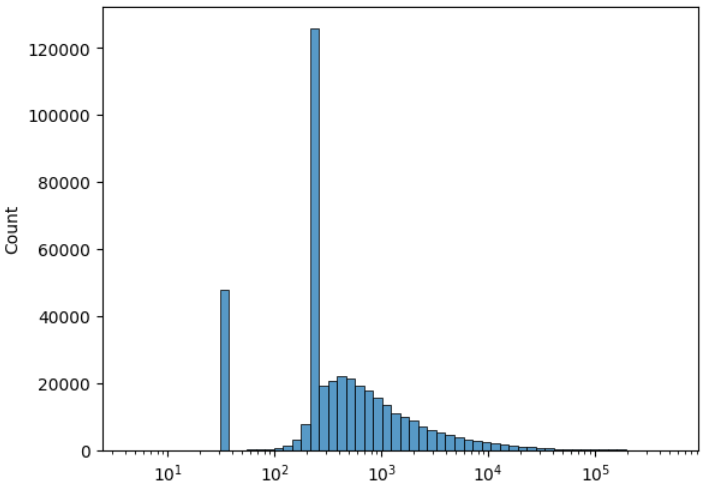
\includegraphics[width=.8\textwidth]{figures/area-dist.png}
    \caption{Distribution of Bounding Boxes' Area}
    \label{fig:areadist}
  \end{figure}

  The distribution of objects position in the camera can be seen on Figure \ref{fig:objectheatmap}
  Most of the objects are around the center of the image.

  \begin{figure}[H]
    \centering
    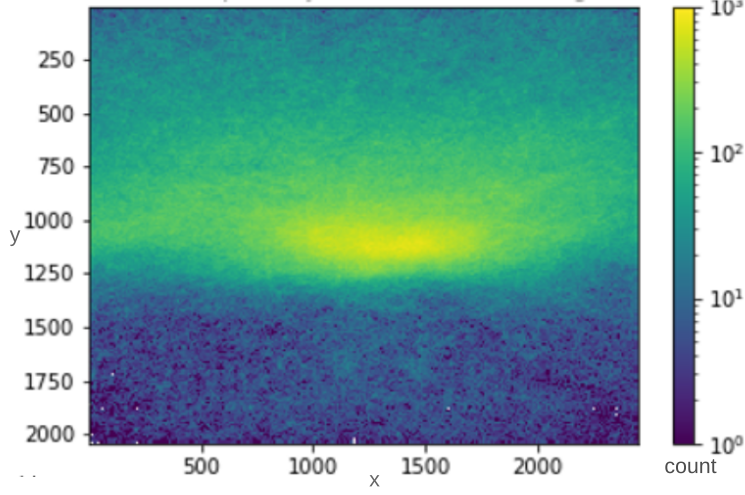
\includegraphics[width=.8\textwidth]{figures/object-pos-dist.png}
    \caption{Distribution of Bounding Boxes' Area \parencite{aot_docs}}
    \label{fig:objectheatmap}
  \end{figure}

  The dataset is structured in the following manner:

  \begin{forest}
  for tree={
    grow'=0,
    child anchor=west,
    parent anchor=south,
    anchor=west,
    calign=first,
    edge path={
      \noexpand\path [draw, \forestoption{edge}]
      (!u.south west) +(7.5pt,0) |- node[fill,inner sep=1.25pt] {} (.child anchor)\forestoption{edge label};
    },
    before typesetting nodes={
      if n=1
        {insert before={[,phantom]}}
        {}
    },
    fit=band,
    before computing xy={l=25pt},
  }
[Data
  [Part1
    [Images
      [FlightSequence1
        [FlightSequence1Timestamp1.png]
        [FlightSequence1Timestamp2.png]
        [...]
      ]
      [FlightSequence2]
      [...]
    ]
    [labels.json]
  ]
  [Part2]
  [Part3]
]
\end{forest}
  
  And each labels JSON file is also structured like this:

  \begin{forest}
  for tree={
    grow'=0,
    child anchor=west,
    parent anchor=south,
    anchor=west,
    calign=first,
    edge path={
      \noexpand\path [draw, \forestoption{edge}]
      (!u.south west) +(7.5pt,0) |- node[fill,inner sep=1.25pt] {} (.child anchor)\forestoption{edge label};
    },
    before typesetting nodes={
      if n=1
        {insert before={[,phantom]}}
        {}
    },
    fit=band,
    before computing xy={l=25pt},
  }
[Samples
  [FlightSequence1
    [Entities
    [Entity1
      [Timestamp]
      [ImageName]
      [BoundingBox
        [class]
        [{x1,y1,x2,y2}]
      ]
    ]
    [Entity2]
    [...]
    ]
  ]
  [FlightSequence2]
  [...]
]
\end{forest}
  
  Notice that the labels are structured entity based. This made the label convertion process
  more complex. This topic will be discussed more in the next section.


  \subsection{Dataset Sampling}
  \label{section:datasetsampling}
    \subsubsection{Sampling Distribution}
    As seen on section \ref{section:datasetsource}, The size of the dataset is massive.
    For this reason, we only downloaded the planned encounters from the AWS S3 Bucket which 
    in total amounted to 1.1 TB. As this number is still too large
    due to the limitation of computational resource, we will only sample some of them
    for training and testing. We will sample in total 700 images from the dataset with splits
    as shown in Table \ref{tbl:datasetsamplingdist}.
    %Karena jumlah dataset pada \textcite{aot_dataset} berukuran sangat besar, dan keterbatasan
    %\emph{computational resource}, hanya sebagian dari dataset tersebut akan digunakan untuk \emph{training} dan \emph{test}.
    %Akan diambil total 700 gambar dari dataset dengan pembagian sesuai dengan Tabel \ref{tbl:datasetsamplingdist}
    \begin{table}[H]
      \centering
      \captionof{table}{Distribusi Sampling Dataset}
      \label{tbl:datasetsamplingdist}
      
\begin{tabular}{c c c c c c c}
  \toprule[1.5pt]
  Splits    &Total &\multicolumn{5}{c}{Classes Percentage}\\
%                    \cline{3-7}
            &Images& Airplane & Helicopter & Bird & Drone & Negative\\
  \midrule
  Training  &400   &23.75\%   &23.75\%     &23.75\% &23.75\%       &5\%\\
  \midrule
  Validation&100   &20\%      &20\%        &20\%    &20\%          &20\%\\
  \midrule
  Test      &200   &20\%      &20\%        &20\%    &20\%          &20\%\\
  \bottomrule[1.5pt]
\end{tabular}
    \end{table}
    
    \subsubsection{Sampling and Label Convertion Procedure}
    Sampling the dataset was not straightforward. Due to how the \textcite{aot_dataset} files and labels was structured,
    we had to make a sampling and converting procedure like the following:

    \begin{enumerate}
      \item Open all \verb|labels.json| file and load all entities into a single list called \verb*|entities|
      \item Let \verb|Img2Boxes| be a dictionary with image names as key and list of bounding boxes in the image as value.
      \item Let \verb|Cls2Img| be a dictionary with 4 class names as key (airplane, bird, etc) and set of image name that contain object of those classes as the value.
      \item Populate \verb|Img2Boxes| and \verb|Cls2Img| in the following manner:
      \begin{lstlisting}
      For entity in entities:
        Img2Boxes[entity.ImageName].append(entity.BoundingBox)
        Cls2Img[entity.BoundingBox.class].append(entity.ImageName)
      \end{lstlisting}
      \item Calculate the total image needed for each class according to Table \ref{tbl:datasetsamplingdist}.\\
            e.g. Total image needed for airplane class is $\frac{400\times 23.75+100\times 20+200\times 20}{100}$.
      \item Distribute the images to train, valid and test.
      \begin{lstlisting}
      For class in list_of_classes:
        Images[class] = Cls2Img[class].random_choice(TotalImageNeeded[class])
      For class in list_of_classes[-1]: // except negative sample
        addtotrain = images[class][:23.75/63.75*TotalImageNeeded[class]]
        images[class] = images[class][23.75/63.75*TotalImageNeeded[class]:]
        train.append(addtotrain)

        do the same to valid and test
      process the negative sample independently
        

      
      \end{lstlisting}
    
      \item Convert \verb|train|, \verb|valid|, \verb|test| to darknet format.
      \begin{lstlisting}
      For img in train:
        label = []
        For boxes in Img2Boxes[img]
          // to_darknet converts class xyxy to class x y w h normalized
          label.append(to_darknet(boxes.BoundingBox))
        copy(img, train_folder+img)
        write(label, train_folder+img.with_suffix('.txt'))

      repeat for valid and test
      \end{lstlisting}

    \end{enumerate}
    %\begin{lstlisting}[caption={Test},mathescape,escapechar=\%]
    %  //Calculate the total image needed for each class (Table %\ref{tbl:datasetsamplingdist}%)
    %  TotalClassesPartition = [$\frac{400*23.75 + 100*20 + 200*20}{100}$].repeat(4) //for each class
    %  TotalClassesPartition.append($\frac{400*5 + 100*20 + 200*20}{100}$) // for negative class


    %\end{lstlisting}
  %Untuk membagi dataset agar terdistribusi seperti pada Tabel \ref{tbl:datasetsamplingdist}, akan digunakan algoritma seperti berikut:
  %\begin{algorithmic}
  %  \State $L_0 \gets$ List index gambar-gambar yang memiliki objek kelas pesawat
  %  \State $L_1 \gets$ List index gambar-gambar yang memiliki objek kelas helikopter
  %  \State $L_2 \gets$ List index gambar-gambar yang memiliki objek kelas burung 
  %  \State $L_3 \gets$ List index gambar-gambar yang memiliki objek kelas \emph{Other}
  %  \State $L_4 \gets$ List index gambar-gambar yang memiliki objek kelas negatif
  %  \For{$i \gets 0$ to $4$}
  %    \State $L_i \gets shuffle(L_i)$
  %  
  %  

  %\end{algorithmic}

%\begin{tabular}{>{\hspace{1em}}l >{\hspace{1pt}}l >{\hspace{3em}}l}
  CPU &       & Intel® Core™ i5-9400F CPU @ 2.90GHz\\
  GPU &       & Nvidia Geforce RTX 2080 Ti\\
      &Memory & 12 GB\\
      &Cuda CC& 7.5\\
  RAM &       & 12 GB\\

\end{tabular}

%\begin{itemize}[noitemsep,topsep=0pt]
%  \item CPU \hfill Intel(R) Core(TM) i5-9400F CPU @ 2.90GHz
%  \item GPU \hfill Nvidia Geforce RTX 2080 Ti
%  \begin{itemize}[noitemsep,topsep=0pt]
%    \item[] Memory \hfill 12 GB
%    \item[] CUDA Compute Capability \hfill 7.5
%  \end{itemize}
%  \item RAM \hfill 12 GB
%  \item Disk Available Memory \hfill 1.3 TB
%  \item Operating System \hfill Ubuntu 20.04
%  \item Cuda Toolkit Version \hfill 11.7
%  \item PyTorch Version \hfill 1.13.1
%\
  %Untuk melaksanakan eksperimen ini, akan digunakan suatu komputer yang dilengkapi dengan
  %GPU Nvidia RTX 2080 Ti yang memiliki kapasitas 11GB VRAM. Oleh karena keterbatasan ini,
  %Melatih model-model YOLOv7 besar seperti W6, E6, dan E2E yang dimodifikasi menjadi sangat sulit,
  %apalagi pada skala input sesuai dengan dimensi dataset.
  %Oleh karena hal ini, arsitektur yang akan dipilih sebagai \emph{baseline} modifikasi adalah YOLOv7 dengan
  %ukuran normal karena model tersebut adalah model terbesar yang mampu di-\emph{train} pada RTX 2080 Ti dengan 
  %input size 1600x1600 dan batch size 1.

  %Selain itu, jumlah dataset yang akan digunakan juga akan dibatasi menjadi 400 seperti pada subbab \ref{section:dataset} untuk menghemat waktu training.
  %Pada pilot test, ditemukan bahwa dibutuhkan sekitar 20 jam untuk men-\emph{train} model sebanyak 300 epoch pada dataset dengan 400 gambar jika menggunakan
  %GPU RTX 2080 Ti.

%\section{Setting Up Experiment Environment}
%
%  \subsection{Training System}
%  \subsection{Pilot Test}
  %\subsection{Pilot Test}





%\section{Skema Training Model}
%  Untuk melatih berbagai modifikasi YOLOv7, akan dibuat suatu \emph{auto-trainer}.
%  \emph{Auto-trainer} ini akan menerima suatu \emph{file} konfigurasi modifikasi YOLOv7, dan dengan otomatis membangun arsitektur YOLOv7 yang termodifikasi dan melatihnya.
%  Setelah mendapatkan model modifikasi YOLOv7 yang sudah dilatih, \emph{auto-trainer} akan menguji model tersebut dengan dataset uji.
%  Metrik-metrik pengujian, grafik histori \emph{training loss vs validation loss}, dan \emph{weights} dari model kemudian akan dikirim ke user.
%  Dengan membuat \emph{auto-trainer} ini, proses pelatihan model dan pelaporan hasil menjadi terotomasi sehingga akan mempermudah proses penelitian.
%
%\section{Timeline Pelaksanaan Penelitian}
%  \newcommand{\w}{}
%  \newcommand{\G}{\cellcolor{gray}}
%  \begin{table}[h!]
%    \captionof{table}{Tabel timeline}
%    \label{tbl:timeline}
%    \begin{tabular}{|p{3.5cm}|c|c|c|c|c|c|c|c|c|c|c|c|c|c|c|c|}
%  
%      \hline
%      \multirow{2}{*}{Kegiatan} & \multicolumn{16}{|c|}{Minggu} \\
%      \cline{2-17} &
%      1 & 2 & 3 & 4 & 5 & 6 & 7 & 8 & 9 & 10 & 11 & 12 & 13 & 14 & 15 & 16 \\
%      \hline
%  
%      % Gunakan \G untuk mengisi sel dan \w untuk mengosongkan sel
%      Persiapan Dataset &
%      \G & \w & \w & \w & \w & \w & \w & \w & \w & \w & \w & \w & \w & \w & \w & \w \\
%      \hline
%  
%      Pemb. \emph{Auto-trainer} &
%      \w & \G & \w & \w & \w & \w & \w & \w & \w & \w & \w & \w & \w & \w & \w & \w \\
%      \hline
%  
%      Pemb. Konfigurasi&
%      \w & \w & \G & \G & \G & \G & \G & \G & \G & \G & \G & \G & \w & \w & \w & \w \\
%      Modifikasi &
%      \w & \w & \G & \G & \G & \G & \G & \G & \G & \G & \G & \G & \w & \w & \w & \w \\
%      \hline
%  
%      Training Model &
%      \w & \w & \G & \G & \G & \G & \G & \G & \G & \G & \G & \G & \w & \w & \w & \w \\
%      \hline
%
%      Analisis &
%      \w & \w & \G & \G & \G & \G & \G & \G & \G & \G & \G & \G & \G & \w & \w & \w \\
%      \hline
%
%      Pemb. Laporan &
%      \w & \w & \w & \w & \w & \w & \w & \w & \w & \w & \w & \w & \G & \G & \G & \G \\
%      \hline
%  
%    \end{tabular}
%  \end{table}
